\begin{enumerate}[label=\thesection.\arabic*, ref=\thesection.\theenumi]
	\item Take a board marked from -104 to 104 as shown in 
  \tabref{tab:game}.  
	\begin{table}[H]
%  \centering
  %\documentclass{article}
%\usepackage{tikz}
%\usepackage[table]{xcolor}
%\usepackage[margin=1in]{geometry}
%\usepackage{array}
%\usepackage{graphicx}


%\begin{document}

\begin{center}
\begin{tikzpicture}
% Draw the table
\node (tbl) at (0, 0) {
\renewcommand{\arraystretch}{1.2}
\setlength{\tabcolsep}{6pt}
\arrayrulewidth=0.4pt
\begin{tabular}{|*{11}{>{\columncolor{lightblue}}c|}}
%\begin{tabular}{|*{11}{c|}}
\hline
104 & 103 & 102 & 101 & 100 & 99  & 98  & 97  & 96  & 95  & 94  \\
\hline
83  & 84  & 85  & 86  & 87  & 88  & 89  & 90  & 91  & 92  & 93  \\
\hline
82  & 81  & 80  & 79  & 78  & 77  & 76  & 75  & 74  & 73  & 72  \\
\hline
61  & 62  & 63  & 64  & 65  & 66  & 67  & 68  & 69  & 70  & 71  \\
\hline
60  & 59  & 58  & 57  & 56  & 55  & 54  & 53  & 52  & 51  & 50  \\
\hline
39  & 40  & 41  & 42  & 43  & 44  & 45  & 46  & 47  & 48  & 49  \\
\hline
38  & 37  & 36  & 35  & 34  & 33  & 32  & 31  & 30  & 29  & 28  \\
\hline
17  & 18  & 19  & 20  & 21  & 22  & 23  & 24  & 25  & 26  & 27  \\
\hline
16  & 15  & 14  & 13  & 12  & 11  & 10  & 9   & 8   & 7   & 6   \\
\hline
-5  & -4  & -3  & -2  & -1  & 0   & 1   & 2   & 3   & 4   & 5   \\
\hline
-6  & -7  & -8  & -9  & -10 & -11 & -12 & -13 & -14 & -15 & -16 \\
\hline
-27 & -26 & -25 & -24 & -23 & -22 & -21 & -20 & -19 & -18 & -17 \\
\hline
-28 & -29 & -30 & -31 & -32 & -33 & -34 & -35 & -36 & -37 & -38 \\
\hline
-49 & -48 & -47 & -46 & -45 & -44 & -43 & -42 & -41 & -40 & -39 \\
\hline
-50 & -51 & -52 & -53 & -54 & -55 & -56 & -57 & -58 & -59 & -60 \\
\hline
-71 & -70 & -69 & -68 & -67 & -66 & -65 & -64 & -63 & -62 & -61 \\
\hline
-72 & -73 & -74 & -75 & -76 & -77 & -78 & -79 & -80 & -81 & -82 \\
\hline
-93 & -92 & -91 & -90 & -89 & -88 & -87 & -86 & -85 & -84 & -83 \\
\hline
-94 & -95 & -96 & -97 & -98 & -99 & -100 & -101 & -102 & -103 & -104 \\
\hline
\end{tabular}
};

% Add arrows (approximated based on image)
%\draw[->, thick] (-6.5,4.5) -- ++(-0.6,0);   % Top-left arrow (row 2)
%\draw[->, thick] (-6.5,3.5) -- ++(-0.6,0);   % Row 3
%\draw[->, thick] (-6.5,2.5) -- ++(-0.6,0);   % Row 4
%\draw[->, thick] (-6.5,1.5) -- ++(-0.6,0);   % Row 5
%\draw[->, thick] (-6.5,-1.5) -- ++(0.6,0);   % Row 11
%\draw[->, thick] (-6.5,-2.5) -- ++(0.6,0);   % Row 12
%\draw[->, thick] (-6.5,-3.5) -- ++(0.6,0);   % Row 13
%\draw[->, thick] (-6.5,-4.5) -- ++(0.6,0);   % Row 14
%\draw[->, thick] (-6.5,-5.5) -- ++(0.6,0);   % Row 15
%\draw[->, thick] (-6.5,-6.5) -- ++(0.6,0);   % Row 16

\end{tikzpicture}
\end{center}

%\end{document}


  \caption{}
  \label{tab:game}
\end{table}
	\item Take a bag containing two blue and two red dice.  Number of dots on the blue dice indicate positive integers and number of dots on the red dice indicate negative integers.
	\item Every player will place his/her counter at zero.
	\item Each player will take out two dice at a time from the bag and throw them.
	\item After every throw, the player has to multiply the numbers marked on the dice.
	\item If the product is a positive integer then the player will move his counter towards 104; if the product is a negative integer then the player will move his counter towards -104.
	\item The player who reaches either -104 or 104 first is the winner.
		\iffalse
		\begin{figure}[H]
  \centering
  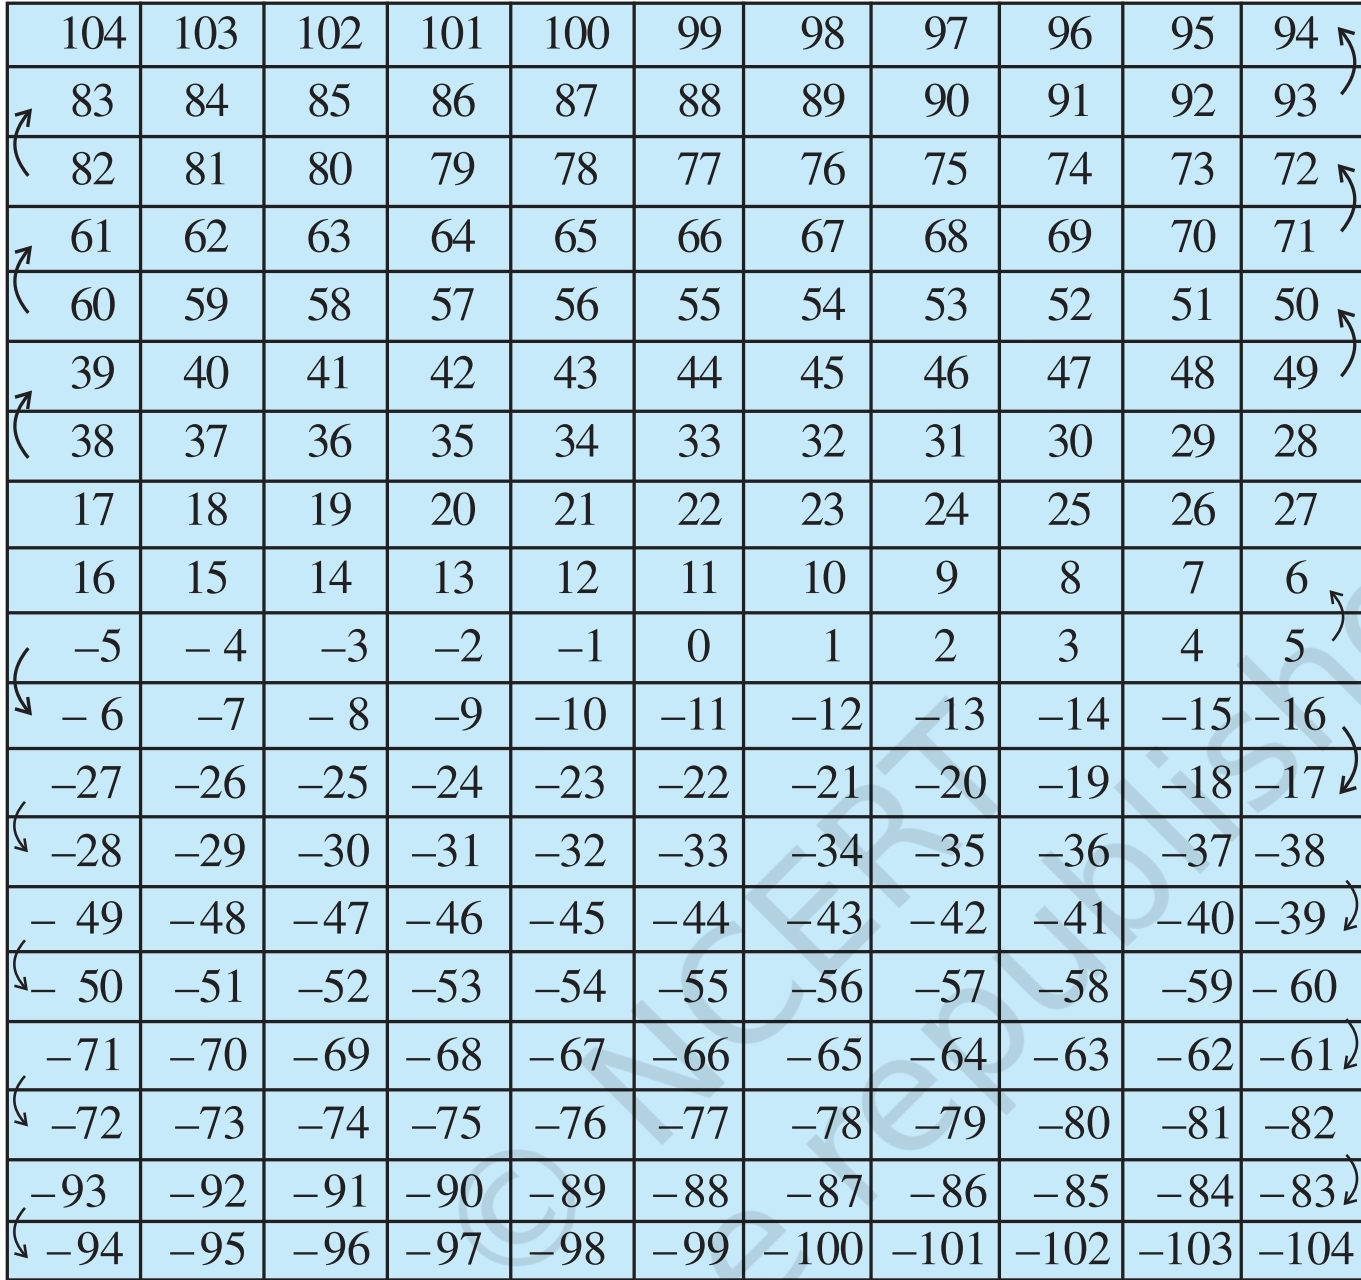
\includegraphics[width=\columnwidth]{figs/game1.jpg}
  \caption{}
  \label{fig:game1}
\end{figure}
\fi
\end{enumerate}
%
\begin{enumerate}[label=\thesection.\arabic*, ref=\thesection.\theenumi,resume*]
	\item Write a program to simulate the game.  Give the inputs manually.
	\\
	\solution 
	\lstinputlisting{codes/rv/game.c}
	\item Revise the program by replacing the second player with the computer.  The computer generates the inputs randomly as follows 
		\begin{enumerate}
			\item Generate the numbers on all the dice using a uniform distribution ranging from 1 to 6.
			\item Simulate the blue and red dice through a Bernoulli distribution having values 1 and -1.
		\end{enumerate}
	\solution 
	\lstinputlisting{codes/rv/rgame.c}
\item Now revise the program so that both players are simulated by the computer.
\end{enumerate}
